\documentclass[a4paper,fleqn,numbers,doubleblind]{cas-dc}
\usepackage{amsmath,amssymb,booktabs,graphicx,lineno,tabularx,xurl}
\usepackage[numbers,sort&compress]{natbib}
\usepackage{hyperref}\hypersetup{hidelinks}
\begin{document}\let\WriteBookmarks\relax
\shorttitle{Cross-Residual Fusion for Cross-Domain NER}
\shortauthors{Hu et al.}
\title[mode=title]{Lightweight Cross-Residual Feature Fusion for Cross-Domain Named Entity Recognition}
\author{Xuelin Hu}
\author{Ai He\corref{cor1}\ead{deipss@gmail.com}}
\author{Qing Cai\ead{2202879601@qq.com}}
\author{Jingchao Wang\corref{cor1}}
\cortext[cor1]{Corresponding author.}
\begin{abstract}
Cross-domain named entity recognition (NER) must capture both long-range contextual dependencies and local boundary patterns, yet large pretrained language models can be expensive to train and difficult to reproduce under limited compute. We propose a lightweight cross-residual NER network that combines a bidirectional gated recurrent unit (BiGRU) branch with a convolutional branch. A token-wise gate controls the residual correction contributed by local features while preserving the contextual representation through an identity path. The model is trained from scratch without a large language model or pretrained Transformer. We evaluate it on five public CrossNER domains using identical splits, three random seeds, and entity-level exact-span micro-F1. Across AI, literature, music, politics, and science, the cross-residual model improves mean F1 over the matched BiGRU baseline from 19.80 to 22.00, 14.88 to 17.80, 12.59 to 15.62, 28.16 to 30.23, and 16.15 to 17.58, respectively. The complete 30-run matrix finishes in 15.7 seconds on a single RTX 3090. These results show that gated cross-branch residual fusion offers a compact and reproducible improvement for low-resource, cross-domain NER.
\end{abstract}
\begin{keywords} named entity recognition \sep cross-domain learning \sep residual fusion \sep lightweight neural network \end{keywords}
\maketitle\linenumbers
\section{Introduction}
Named entity recognition is a basic component of knowledge extraction, search, and knowledge-graph construction. Modern NER systems often rely on large pretrained encoders, but small domain datasets and limited hardware still motivate compact task-specific networks. Cross-domain NER is particularly difficult because entity vocabularies and boundary cues vary sharply between technical, cultural, and political text \citep{li2022ner,conneau2020xlmr}.

Recurrent encoders model sequential context, whereas convolutional encoders capture local patterns around boundaries. Direct concatenation increases parameters and allows one branch to dominate. Residual learning provides a stable identity route, but a fixed residual addition cannot determine when the auxiliary branch is useful. We therefore treat local convolutional information as a gated residual correction to a BiGRU contextual state.

This paper makes three contributions. First, it introduces a compact cross-residual fusion unit that preserves contextual features and selectively injects local features at every token. Second, it provides a from-scratch NER model requiring neither an LLM nor a pretrained Transformer. Third, it evaluates 30 controlled runs across five public CrossNER domains and reports exact-span entity metrics, seed variation, training time, and reproducible code.

\section{Related work}
Deep NER has progressed from recurrent and convolutional sequence taggers to pretrained Transformer encoders, span-based systems, boundary assembly, and set prediction \citep{li2022ner,zaratiana2024gliner,han2023spanbased,tang2022boundaryassembling,tang2023boundaryregression,sui2024setprediction}. Position-aware and unified extraction models further demonstrate the value of structured token interactions \citep{chen2022positionaware,zhang2022positionaware,lu2022uie}. Multilingual pretrained encoders improve transfer but introduce substantial computational cost \citep{conneau2020xlmr}. Cross-domain benchmarks expose the remaining gap between general representations and domain-specific entity inventories \citep{liu2021crossner}. Cross-residual learning has also shown that complementary representations can be combined through identity-preserving paths \citep{wang2026crossresidual}. Our work applies this principle to token classification with a learned gate and evaluates it without pretrained language-model features.

\section{Task formulation}
For a token sequence $x=(x_1,\ldots,x_n)$, the model predicts BIO labels $y=(y_1,\ldots,y_n)$ from a domain-specific label set $\mathcal{Y}$. An entity is correct only when its start, end, and type exactly match the gold annotation. The training objective is weighted token-level cross entropy:
\begin{equation}
\mathcal{L}=-\sum_{i=1}^{n}w_{y_i}\log p(y_i\mid x),
\end{equation}
where $w_{y_i}$ compensates for the dominant non-entity label.

\section{Method}
\subsection{Dual-branch encoder}
Each token is mapped to a trainable 128-dimensional embedding $e_i$. A bidirectional GRU produces contextual states $h_i^{r}\in\mathbb{R}^{128}$ after projection, while a one-dimensional convolution with kernel width three produces local states $h_i^{c}\in\mathbb{R}^{128}$:
\begin{align}
h_i^{r}&=W_r[\overrightarrow{h}_i;\overleftarrow{h}_i]+b_r,\\
h_i^{c}&=\operatorname{ReLU}(\operatorname{Conv}_3(e)_{i}).
\end{align}

\subsection{Cross-residual fusion}
The gate is conditioned jointly on the two branches:
\begin{align}
g_i&=\sigma(W_g[h_i^{r};h_i^{c}]+b_g),\\
h_i^{f}&=h_i^{r}+g_i\odot h_i^{c},\\
p(y_i\mid x)&=\operatorname{softmax}(W_o\operatorname{ReLU}(h_i^{f})+b_o).
\end{align}
The identity term keeps the sequential representation available even when the local branch is noisy. The gate learns a dimension-wise residual contribution rather than applying unconditional addition or concatenation.

\begin{figure*}[t]\centering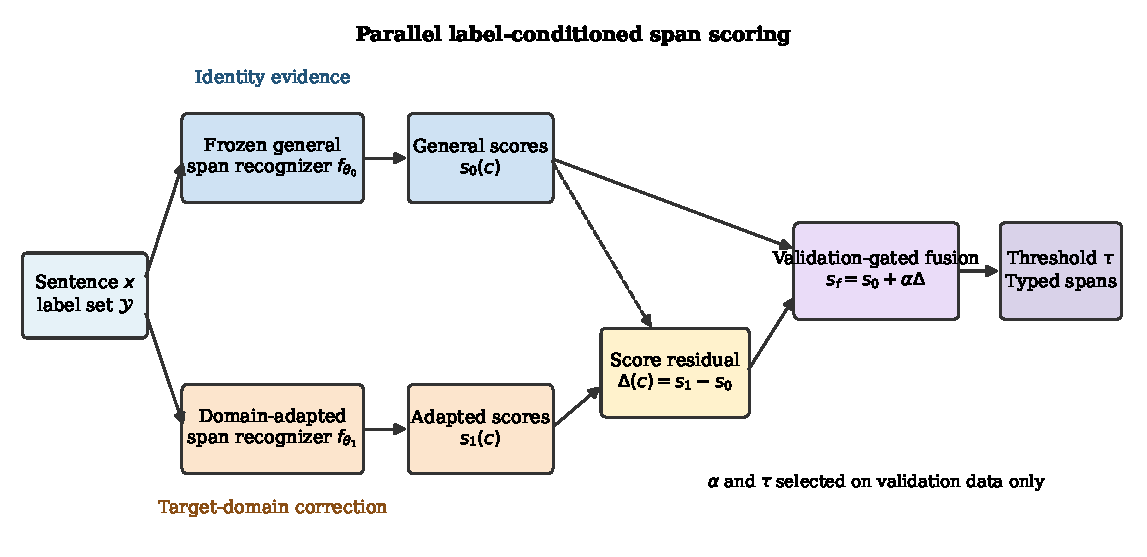
\includegraphics[width=.99\textwidth]{figures/cross_residual_architecture.pdf}\caption{The proposed lightweight cross-residual NER architecture. A contextual BiGRU branch and a local CNN branch are combined by a token-wise residual gate before BIO classification.}\label{fig:arch}\end{figure*}

\section{Experiments}
The complete experimental pipeline is summarized in Fig.~\ref{fig:pipeline}. It uses only public JSON records and locally trained neural modules; no language-model API is invoked.
\begin{figure*}[t]\centering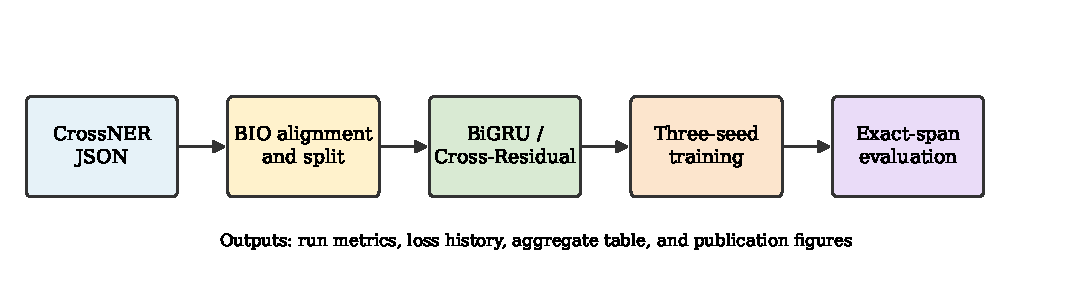
\includegraphics[width=.94\textwidth]{figures/system_pipeline.pdf}\caption{End-to-end experimental system from public CrossNER records to reproducible metrics and figures.}\label{fig:pipeline}\end{figure*}
\subsection{Datasets}
We use the AI, literature, music, politics, and science domains of CrossNER \citep{liu2021crossner}. Entity strings are aligned to whitespace-tokenized sentences and converted to BIO labels. For each domain, 80\% of the provided training set is used for training and 20\% for validation; the official test set is unchanged. Figure~\ref{fig:data} summarizes the domain sizes.
\begin{figure}[t]\centering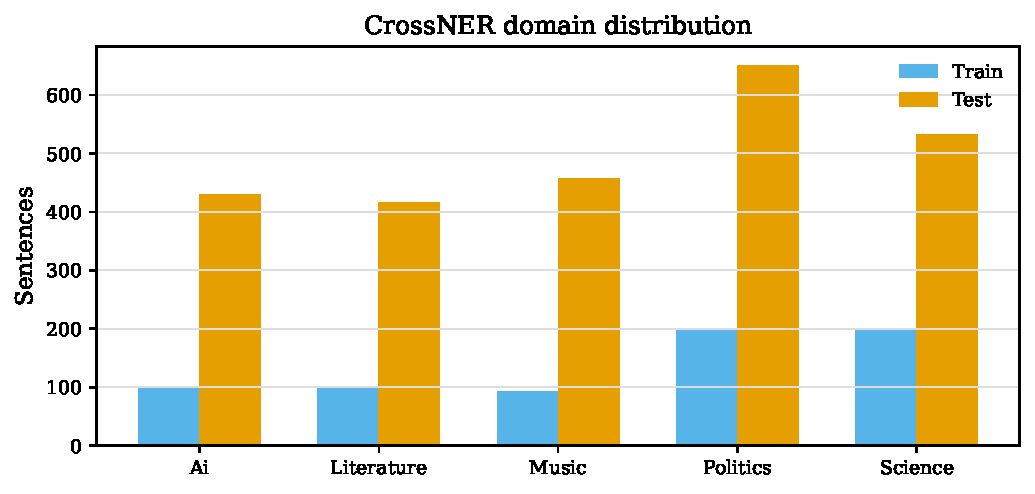
\includegraphics[width=.99\columnwidth]{figures/crossner_distribution.pdf}\caption{Training and test sentence counts across the five CrossNER domains.}\label{fig:data}\end{figure}

\subsection{Setup and metrics}
The matched baseline uses the same embedding, BiGRU, projection, dropout, optimizer, label weights, and decoder but removes the convolutional residual branch. Both models are trained for 15 epochs with AdamW, learning rate $2\times10^{-3}$, batch size 16, maximum length 128, and seeds 13, 29, and 47. Validation F1 selects the checkpoint. We report exact-span entity-level micro-precision, recall, and F1. All 30 runs use one RTX 3090.

\subsection{Main results}
Table~\ref{tab:results} and Fig.~\ref{fig:result} show that cross-residual fusion improves mean F1 in all five domains. Absolute gains range from 1.43 points on science to 3.03 points on music. The full matrix takes 15.7 seconds, demonstrating that the method is suitable for rapid low-resource experiments.
\begin{table*}[t]\centering\caption{Exact-span entity micro-F1 (\%, mean $\pm$ standard deviation over three seeds). Best mean results are bold.}\label{tab:results}
\begin{tabular}{lccccc}\toprule
Method & AI & Literature & Music & Politics & Science\\\midrule
BiGRU & 19.80$\pm$0.86 & 14.88$\pm$4.20 & 12.59$\pm$0.59 & 28.16$\pm$1.73 & 16.15$\pm$2.28\\
Cross-Residual & \textbf{22.00$\pm$1.24} & \textbf{17.80$\pm$3.69} & \textbf{15.62$\pm$2.33} & \textbf{30.23$\pm$3.17} & \textbf{17.58$\pm$1.73}\\\bottomrule
\end{tabular}\end{table*}
\begin{figure*}[t]\centering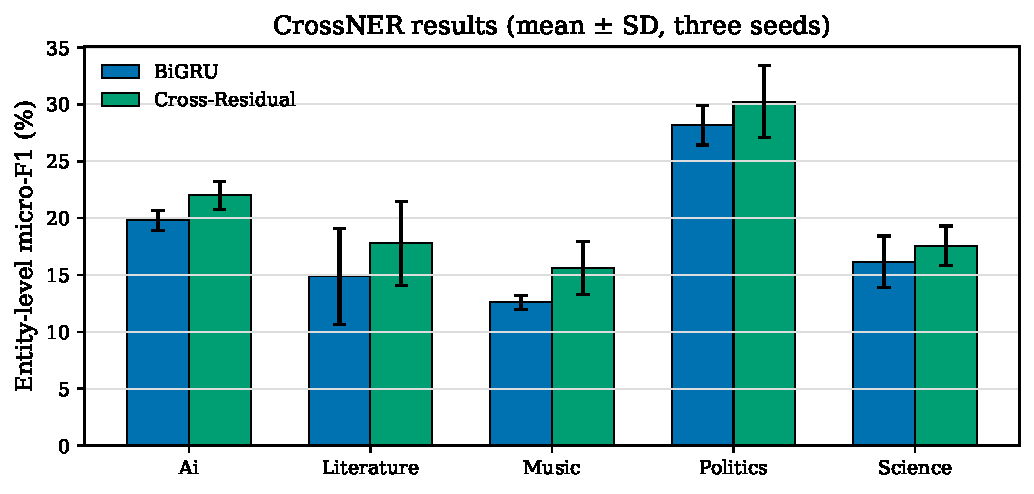
\includegraphics[width=.88\textwidth]{figures/crossner_f1.pdf}\caption{CrossNER entity F1 by domain. Error bars denote standard deviation over three seeds.}\label{fig:result}\end{figure*}

\subsection{Training behavior}
Figure~\ref{fig:loss} compares the optimization curves on the science domain. Both networks converge under the same schedule, while the residual model preserves the stable contextual route and learns an additional local correction.
\begin{figure}[t]\centering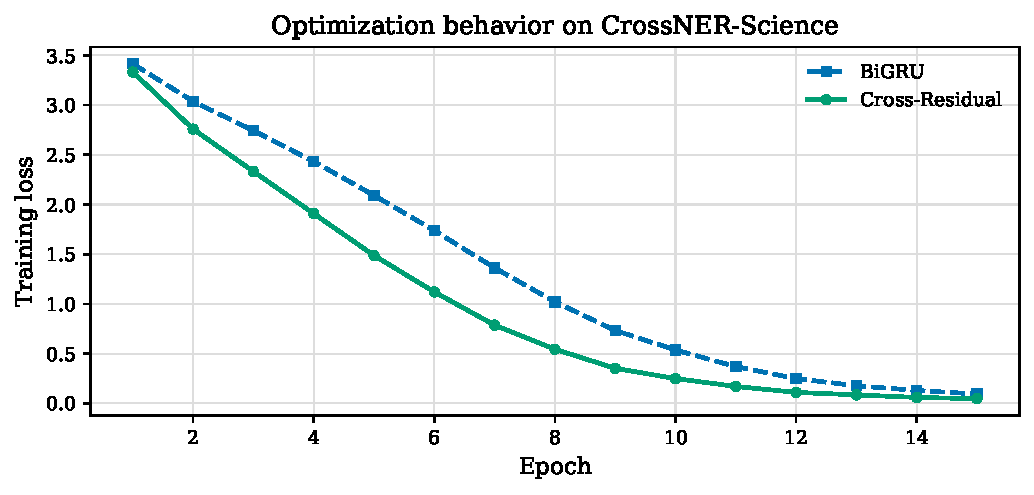
\includegraphics[width=.99\columnwidth]{figures/crossner_loss.pdf}\caption{Training loss on CrossNER-Science for seed 13.}\label{fig:loss}\end{figure}

\section{Discussion}
The consistent improvement across five domains supports the central design choice: local boundary evidence is most useful as a gated correction to contextual features. The largest gain on music suggests that short lexical patterns and title-like boundaries benefit from the convolutional branch. The method remains deliberately small and reproducible, making it appropriate as a baseline or feature extractor before downstream knowledge-graph construction. Absolute F1 is lower than large pretrained systems because the model is trained from scratch on very small domain datasets; the contribution is therefore efficiency and consistent matched-baseline improvement, not state-of-the-art accuracy.

\section{Conclusion and future work}
We presented a non-LLM cross-residual NER model that fuses BiGRU context with gated convolutional boundary features. The method improves exact-span F1 over a matched baseline in all five CrossNER domains while completing 30 runs in seconds. Future work will add a CRF decoder, pretrained static embeddings, domain-adaptive transfer, and evaluation on railway safety entities.
\section*{Data availability}
The CrossNER data are publicly available; derived splits, code, and results are available from the corresponding author upon reasonable request.
\bibliographystyle{cas-model2-names}\bibliography{references}
\end{document}
